\documentclass[11pt]{report}
\usepackage[utf8]{inputenc}
\usepackage[danish]{babel}
\usepackage [T1]{fontenc}
\usepackage[margin=2.5cm]{geometry}
\usepackage[hidelinks]{hyperref}
\usepackage{graphicx}
\graphicspath{{Img/}}
\usepackage{listings}
\usepackage{color}
\usepackage{adjustbox}
\usepackage{tocloft}
\usepackage{listings}
\usepackage{enumitem}
\usepackage{indentfirst}
\usepackage{caption}
\usepackage{float}

\setlength{\parskip}{12pt}

\definecolor{dkgreen}{rgb}{0,0.6,0}
\definecolor{gray}{rgb}{0.5,0.5,0.5}
\definecolor{mauve}{rgb}{0.58,0,0.82}

\lstset{frame=tb,
  language=Java,
  aboveskip=3mm,
  belowskip=3mm,
  showstringspaces=false,
  columns=flexible,
  basicstyle={\small\ttfamily},
  numbers=none,
  numberstyle=\tiny\color{gray},
  keywordstyle=\color{blue},
  commentstyle=\color{dkgreen},
  stringstyle=\color{mauve},
  breaklines=true,
  breakatwhitespace=true,
  tabsize=3
}

\definecolor{bluekeywords}{rgb}{0.13,0.13,1}
\definecolor{greencomments}{rgb}{0,0.5,0}
\definecolor{turqusnumbers}{rgb}{0.17,0.57,0.69}
\definecolor{redstrings}{rgb}{0.5,0,0}


\lstdefinelanguage{FSharp}
                {morekeywords={let, new, match, with, rec, open, module, namespace, type, of, member, and, for, in, do, begin, end, fun, function, try, mutable, if, then, else},
    keywordstyle=\color{bluekeywords},
    sensitive=false,
    morecomment=[l][\color{greencomments}]{///},
    morecomment=[l][\color{greencomments}]{//},
    morecomment=[s][\color{greencomments}]{{(*}{*)}},
    morestring=[b]",
    stringstyle=\color{redstrings}
    }
\usepackage{amsmath}

\title{Social Engineering\\Security}
\author{
Asger H. Sørensen\\
\\cph-as466
\and
William S. Huusfeldt\\
\\cph-wh143
\and
Emil J. Svensmark\\
\\cph-eb122
}
\date{29 - maj - 2020}
\begin{document}
\maketitle
\renewcommand{\cftchapleader}{\cftdotfill{\cftdotsep}}
\tableofcontents
\newpage

\chapter*{1. Indledning}
\addcontentsline{toc}{chapter}{1. Indledning}
Denne rapport vil omhandle et ofte overset område af cybersikkerhed: den humane faktor. I denne rapport indgår eksempler på phishing og vishing. Ved at analysere firmaer og privates håndtering af det når det forekommer. Der vil blive lavet test-baseret vishing forsøg på virksomheder og test-baseret phishing forsøg på private folk, hvorefter handlingerne på dem hver i sær vil blive analyseret. I rapporten vil disse handlinger og forbehold også blive diskuteret samt eventuelt komme med løsninger/ændringer med målet om at øge sikkerheden, hvis den ikke skulle være tilstrækkelig. Hvis den skulle vise sig at være tilstrækkelig, så vil der diskuteres hvilke forbehold der gør at sikkerheden er stærk nok. 

\begin{center}
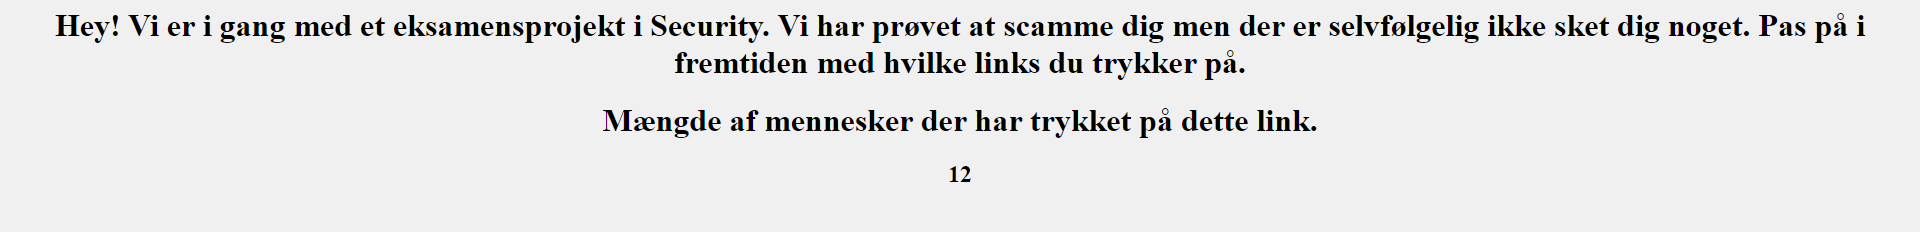
\includegraphics[height=2.5cm, width=17cm]{Capture}
\end{center}

\chapter*{2. Sikkerhed}
\addcontentsline{toc}{chapter}{2. Sikkerhed}

\section*{2. 1 Den Humane Faktor}
\addcontentsline{toc}{section}{2. 1 Den Humane Faktor}

\section*{2. 2 Social Engineering}
\addcontentsline{toc}{section}{2. 2 Social Engineering}

\section*{2. 3 Phishing og man-in-the-middle}
\addcontentsline{toc}{section}{2. 3 Phishing og man-in-the-middle}

\section*{2. 4 Vishing}
\addcontentsline{toc}{section}{2. 4 Vishing}

\chapter*{3. Forsøg}
\addcontentsline{toc}{chapter}{3. Forsøg}

\section*{3. 1 Beskrivelse \& Formål}
\addcontentsline{toc}{section}{3. 1 Beskrivelse \& Formål}

\section*{3. 2 Fremgangsmåde}
\addcontentsline{toc}{section}{3. 2 Fremgangsmåde}

\section*{3. 3 Resultat}
\addcontentsline{toc}{section}{3. 3 Resultat}

\chapter*{4. Refleksion}
\addcontentsline{toc}{chapter}{4. Refleksion}

\chapter*{5. Konklusion}
\addcontentsline{toc}{chapter}{5. Konklusion}

\chapter*{6. Bilag}
\addcontentsline{toc}{chapter}{6. Bilag}

\end{document}